% verslag mod2A
\documentclass{article}
\usepackage[utf8]{inputenc}
\usepackage{float}
\usepackage{graphicx}
\usepackage{amsmath}
\usepackage{amssymb}
\usepackage{amsthm} %nodig voor blokje
\usepackage{marginnote}
\usepackage[outdir=./]{epstopdf}
\usepackage[margin=1in,footskip=0.25in]{geometry} %heb wat meer ruimte
\newcommand\header[1]{\framebox[\linewidth]{\textsc{Opgave #1}}\\}
\newcommand{\Z}{\mathbb{Z}}
\newcommand{\R}{\mathbb{R}}
\newcommand{\Q}{\mathbb{Q}}
\newcommand{\C}{\mathbb{C}}
\newcommand{\N}{\mathbb{N}}
\newcommand{\D}{\partial}

\begin{document}

\section{Average segregation time}
	As mentioned earlier, the segregation time of \(n\%\) is defined as the number of generations until at least \(n\%\) of the population on a board lives in homogenous groups. 
Where person \(i\) is said to live homogenous. If for any neighbour \(j\) of \(i\), we have \(\text{Type}(j)=\text{Type}(i)\).\\
This gives immediate rise to questions concerning the relation between the choice of \(n\) and the average segregation time at \(n\%\). 
Furthermore, it is unclear if segregation at \(n\%\) is guaranteed before a board reaches an equilibrium and what the effect is of the happiness boundary on the existence of a segregation time.\\
\\
To research any of the given questions, we will first have to formalise our choices of board as well as the questions proposed.\\


\subsection{Formalisations}
Prior to starting any test or properly formalising our research questions however, we note that segratation at \(n\%\) does not necessarily have to happen: 
If we consider \(n=100\) on the standard board with happiness \(1/3\). We will nearly never have total segregation before the board reaches an equilibrium.
Therefore one might instead consider the average fraction of segregation at equilibrium,for any given happiness fraction. \\
\\
Furthermore, the average segregation time as function of the segregation fraction should theoretically be a strictly increasing function since for any given board we have:
\begin{align*}
n\% \text{ lives in homogenous groups after } k \text{ generations } \Rightarrow\\
 (n-1)\% \text{ lives in homogenous groups after } k \text{ generations }
\end{align*} 
Having noted these facts, we can now properly formalise the research questions.\\
The following two questions are proposed:
\begin{enumerate}
 \item ***What is the relation between the average segregation time and \(n\).***
 \item What is the average segregated fraction of the population after a board reaches equilibrium for given choices of happiness.
\end{enumerate}

To establish results regarding these questions, we consider different setups in testings. We will be testing two different boards.
The first board to be analysed is the standard board. The second board is a larger 
"4-Type" board. The details are specified below:
\begin{table}[h!]
\centering
\caption{My caption}
\label{my-label}
\begin{tabular}{l|l|l}
  & Standard Board & 4-Type Board\\ \hline
Number of types:& 2 & 4 \\ 
 Length:& 8 & 10  \\
 Width:& 8 & 10  \\
 Happiness:& 1 & 1  \\
Population per type: & 20 & 16  
	\end{tabular}
	\end{table}
\\
The 4-Type board is constructed to maintain the same ratio of inhabited and uninhabited spots as the standard board. The choice of happiness on these boards is 1 unlike the usual \(\frac{1}{3}\). 
This guarantees that for any \(n\leq 100\), segregation at \(n\%\) takes place prior to the board reaching an equilibrium. 
To observe the average segregation time \(n\%\) for any \(n\), 500 simulations will be ran per board and averaged out in order to give an approximation for the average segregation time at \(n\%\).
Likewise the average segregated fraction will be estimate by the average of the segregated fraction of an equilibrium from 500 simulations with given happiness \(q\).
\newpage
\subsection{Results}
The results regarding the first question are shown below:\\

\begin{figure}[H]
    \centering
    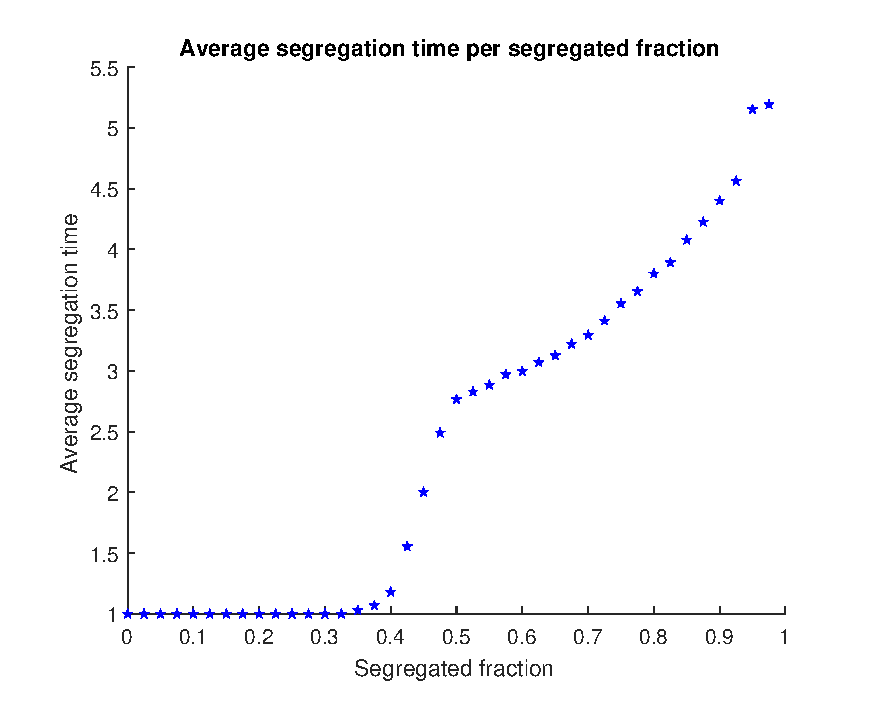
\includegraphics[width=0.8\textwidth]{aveseg_sb_1}
    \caption{Average segregation time on the standard board}
    \label{fig:avesegsb}
\end{figure}

Most notable of figure \ref{fig:avesegsb} is that it is neither linear nor exponential, which is what one might expect. Instead, it appears to be partially exponential and partially lineair. From the figure, we note that the average segregation time increases fastest between 0.4 and 0.5. 
Which is to say that the time it takes three times longer for 50\% of the populations to live in homogenous groups than for 40\%.

 \begin{figure}[H]
    \centering
    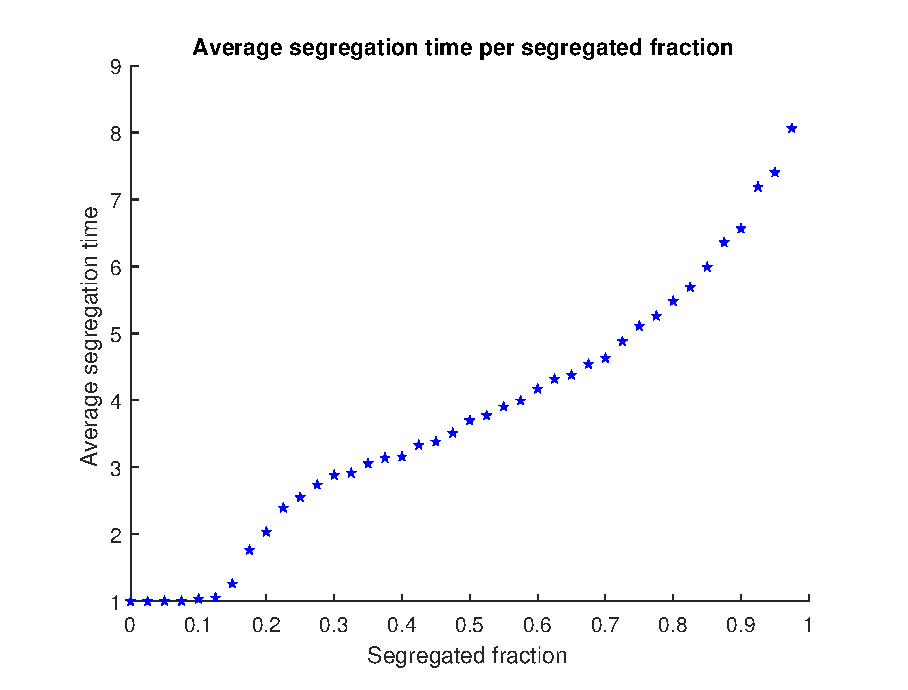
\includegraphics[width=0.8\textwidth]{aveseg_4b_1}
    \caption{Average segregation time on the 4-Type board}
    \label{fig:aveseg4b}
\end{figure}

There is one major differences between the standard board and the 4-type board. 
Namely the fact that there are twices as many types of people in the second model than in the first. Other minor differences include the boardsize.
However the people/boardspace ratio is the same in both models and thus should not have too much of an impact on the results.
The number of types however results in two key differences. The first being the increased number of generations. 
The second (and more interesting) difference is that this graph lifts of earlier. 
This along with the first difference, results in a smoother curve which appears to resemble a cubic relation.

\begin{figure}[H]
    \centering
    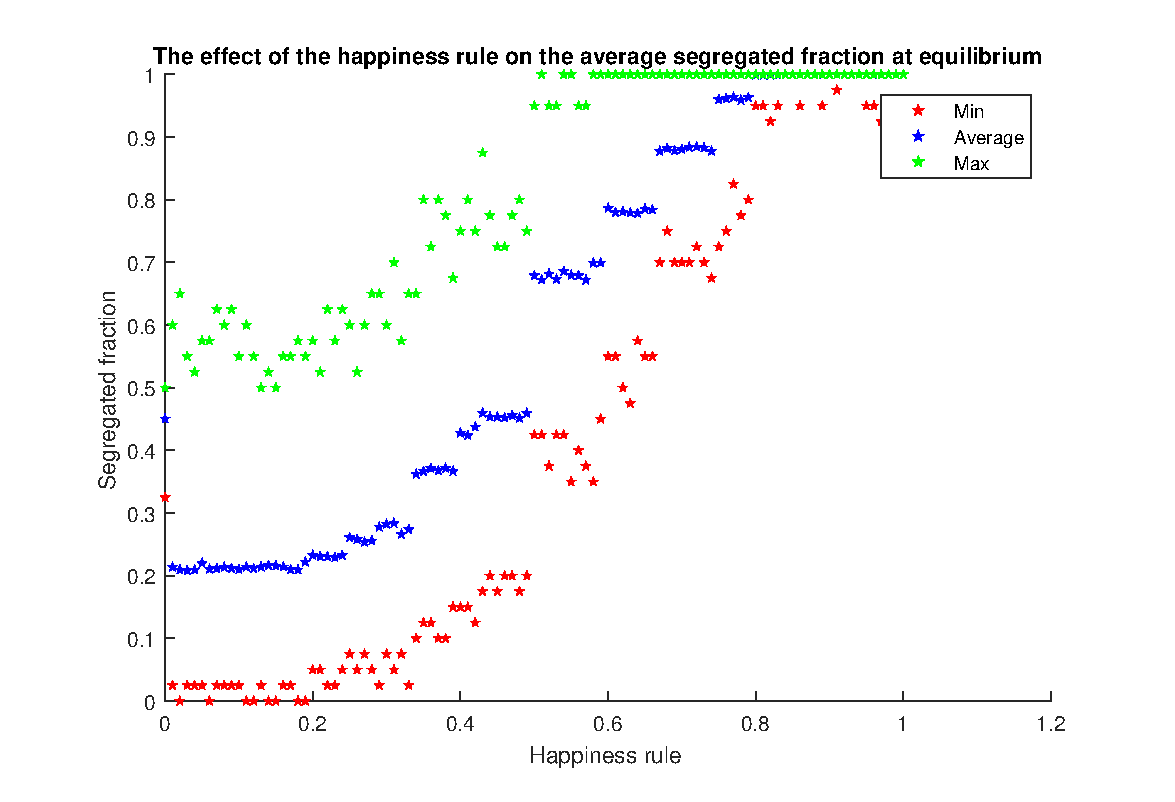
\includegraphics[width=0.8\textwidth]{habysegfrac_sb_1}
    \caption{Average segregated fraction as a result of happiness on the standard board}
    \label{fig:happysegsb}
\end{figure}

Figure \ref{fig:happysegsb} displays three scattered values. The red and green dots represent the minimum and maximum segregrated fraction of 500 boards for the given happiness. Notable in this picture is that the average segregated value is greater than the happiness. 
Another thing worth noting is that the segregated fractions tend to appear in different groups seperated by relatively large percentages.
\section{conclusion?}
\end{document}